% -*- TeX-master: "main"; fill-column: 72 -*-
\section{Package syntax and semantics}

In this section, we define the syntax and semantics of the
\RenderPackage for \sbmlthreecore. We expound on the various data types
and constructs defined in this package, then in \sec{examples}, we
provide complete examples of using the constructs in example SBML
models.

%----------------------------------------
%----------------------------------------
\subsection{Namespace URI and other declarations necessary for using
this package}
\label{xml-namespace}

Every SBML Level~3 package is identified uniquely by an XML namespace
URI. For an SBML document to be able to use a given SBML Level~3
package, it must declare the use of that package by referencing its URI.
The following is the namespace URI for this version of the
\RenderPackage for SBML Level~3 Version~1:

\begin{center}
\uri{http://www.sbml.org/sbml/level3/version1/render/version1}
\end{center}

In addition, SBML documents using a given package must indicate whether
understanding the package is required for complete mathematical
interpretation of a model, or whether the package is optional. This is
done using the attribute \token{required} on the \token{<sbml>} element
in the SBML document. For the \RenderPackage the value of the required
attribute is \val{false}.

The following fragment illustrates the beginning of a typical SBML model
using SBML Level~3 Version~1 and this version of the \RenderPackage (note, that the Layout package is also needed):

\begin{example}
<?xml version="1.0" encoding="UTF-8"?>
 <sbml xmlns="http://www.sbml.org/sbml/level3/version1/core" level="3" version="1"
   xmlns:layout="http://www.sbml.org/sbml/level3/version1/layout/version1" layout:required="false"
   xmlns:render="http://www.sbml.org/sbml/level3/version1/render/version1" render:required="false"
	>
	
\end{example}


Originally the layout and render extension were developed for use with SBML Level 2 files, where the information was stored in annotations to SBML models, layout lists and layouts.
The namespace for the version of the SBML render extension for SBML level 2 is: 

\begin{center}
\uri{http://projects.eml.org/bcb/sbml/render/level2}
\end{center}

An example using the render extension in this context would look like this: 

\begin{example}
<?xml version="1.0" encoding="utf-8"?>
<sbml xmlns="http://www.sbml.org/sbml/level2" level="2" version="1">
  <model id="model1" name="Model with L2 Render Annotation">
    <annotation>
      <listOfLayouts xmlns="http://projects.eml.org/bcb/sbml/level2">
        <layout id="layout1">
          <annotation>
            <listOfRenderInformation xmlns="http://projects.eml.org/bcb/sbml/render/level2">
							...
            </listOfRenderInformation>
          </annotation>
					...
        </layout>
				...
      </listOfLayouts>
			...
    </annotation>
		...
  </model>
</sbml>
\end{example}

%--------------------------------------------------
\subsection{Primitive data types}
\label{primitive-types}

Section~3.1 of the SBML Level~3 specification defines a number of
primitive data types and also uses a number of XML Schema 1.0 data types
\citep{biron:2000}. We assume and use some of them in the rest of this
specification, specifically \primtype{boolean}, \primtype{integer}, \primtype{double}, \primtype{ID},
\primtype{SId}, \primtype{SIdRef}, and \primtype{string}. The
\RenderPackage defines other primitive types; these are described below.

%\TODO{check all necessary types from core are listed}

%-----------------------------------------------
\subsubsection{Type \fixttspace\primtypeNC{StyleType}}

The type \primtype{StyleType} is used by \LocalStyle and \GlobalStyle elements, in order
to apply a particular \Style to a \GraphicalObject. This is done via the \token{typeList} attribute
that uses the \primtype{StyleType} as its data type. 

A valid \StyleType instance is a combination of one or more of the following 
values separated by white spaces:

\begin{itemize}
 \item \val{COMPARTMENT\-GLYPH},
 \item \val{SPECIES\-GLYPH},
 \item \val{REACTION\-GLYPH}, 
 \item \val{SPECIES\-REFERENCE\-GLYPH},
 \item \val{TEXT\-GLYPH}, 
 \item \val{GENERAL\-GLYPH}, 
 \item \val{GRAPHICAL\-OBJECT} 
 \item \val{ANY}
\end{itemize}

The \token{ANY} keyword specifies that this styles applies to any type of glyph and 
would be equivalent to listing all the other keywords. 

%-----------------------------------------------
\subsubsection{Type \fixttspace\primtypeNC{GradientSpreadMethod}}

The type \GradientSpreadMethod is being used by \GradientBase elements to decide how 
gradients propagate over the whole element they are applied to. It is an enumeration consisting 
of the following three values called \texttt{pad}, \texttt{reflect} or \texttt{repeat}:

\begin{itemize}
 \item {\texttt{pad}:} the gradient color at the
endpoint of the vector defines how the gradient is continued beyond that point (default value).
 \item {\texttt{reflect}:} the gradient continues from end to start and
then from start to end again and again.
 \item {\texttt{repeat}:} the gradient pattern is repeated from start to end over and over again.
\end{itemize}

\begin{figure}[!h]
\begin{center}
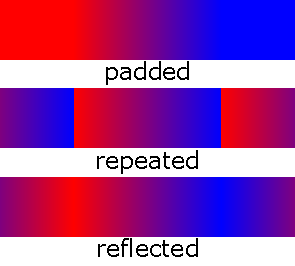
\includegraphics{figures/SVG_spreadMethod.pdf}
\end{center}
\caption{example of different SVG spreadMethod values}
\label{SVG:spreadMethod}
\end{figure}

%-----------------------------------------------
\subsubsection{Type \fixttspace\primtypeNC{FillRule}}

The type FillRule describes how a surface created by connecting 
points on a \Polygon are to be filled when rendered. Allowed values for a valid instance of type \primtype{FillRule} are:

\begin{itemize}
 \item \token{nonzero} 
 \item \token{evenodd}
\end{itemize}

For a detailed description on how these values should be applied, we would like to refer you to the corresponding documentation in the SVG specification  \footnote{ \url{http://www.w3.org/TR/SVG/painting.html\#FillRuleProperty} }. 

%-----------------------------------------------
\subsubsection{Type \fixttspace\primtypeNC{FontFamily}}

The \FontFamily type gives a hint as to which font is to be used when
rendering \Text elements. This type extends the type \primtype{string}. The following values are pre-defined: 

\begin{itemize}
 \item \token{serif}
 \item \token{sans-serif}
 \item \token{monospace}
\end{itemize}

However, applications are free to use the \FontFamily to store the name of the font the writing application used as a string. It has not been a issue for reading applications to find a similar font. 

%-----------------------------------------------
\subsubsection{Type \fixttspace\primtypeNC{FontWeight}}
The type \FontWeight indicates whether the font is to be used in its normal form, or in its bold form. Consequently, the only values allowed for this enumeration are: 

\begin{itemize}
 \item \token{bold} 
 \item \token{normal} 
\end{itemize}

%-----------------------------------------------
\subsubsection{Type \fixttspace\primtypeNC{FontStyle}}

The type \FontStyle determines whether a font is to be
drawn use italic or normal styles. Thus the only allowed values are:

\begin{itemize}
 \item \token{italic} 
 \item \token{normal} 
\end{itemize}

%-----------------------------------------------
\subsubsection{Type \fixttspace\primtypeNC{VTextAnchor}}

The type \VTextAnchor allows models to specify how text elements are to be
vertically aligned within their bounding box. This enumeration has the following allowed values: 

\begin{itemize}
 \item \token{top},
 \item \token{middle}
 \item \token{bottom} 
 \item \token{baseline}
\end{itemize}

Examples illustration the use of the different \VTextAnchor values are given in \apdx{apdx:text-anchor}.

%-----------------------------------------------
\subsubsection{Type \fixttspace\primtypeNC{HTextAnchor}}

The type \HTextAnchor defines the horizontal alignment of text elements. This enumeration can use the following values: 

\begin{itemize}
 \item \token{start}
 \item \token{middle}
 \item \token{end}
\end{itemize}

Examples illustration the use of the different \HTextAnchor values are given in \apdx{apdx:text-anchor}.



%-----------------------------------------------
\subsubsection{Type \fixttspace\primtypeNC{RelAbsVector}}

The position and size of render elements can be specified as a combination of an absolute value and a relative value. The absolute value is a numerical value in units of \val{pt} (1/72 inch) indicating the position of the object. The relative value is a percentage indicating the size of the object. All values are relative to the bounding box of the corresponding element in the layout. This bounding box basically specifies a canvas for the render elements to be drawn on.

In order to avoid populating the resulting XML with numerous attributes the \RenderPackage encodes this information in the \RelAbsVector class with the two attributes \token{abs} and \token{rel} by extending the \primtype{string} such that it encodes optionally an absolute number first followed by an optional 
relative number followed by a \token{\%} sign. Adding spaces between the coordinates is encouraged, but not required.

Examples of the \RelAbsVector construct for the \token{x} coordinate are shown in the table below.
\smallskip
\begin{center}
\begin{tabular}{ | l | p{5cm} |}
\hline
\primtype{string} & Coordinate \\ \hline
$-5+100\%$ & 5 points left of the right edge of the current bounding box.\\ \hline
$50\%$ & 50\% from the left edge of the current bounding box. \\ \hline
$2$ & 2 points from the left edge of the bounding box. \\ 
\hline
\end{tabular}
\end{center}
\smallskip


It should be noted that when applying transformations to elements with relative values, the relative 
values have to be converted to absolute values first.

%-----------------------------------------------
\subsubsection{Type \fixttspace\primtypeNC{doubleArray}}

The \doubleArray primitive type is a comma and space delimited set of \primtype{double} values in a single string as shown in the following example:

\begin{center}
"1.0, 2.1, 3.2, 4.0, 5.3"
\end{center}

%-----------------------------------------------
\subsubsection{Type \fixttspace\primtypeNC{colorString}}

The \colorString primitive type is a string encoding the hexidecimal color code. Color values are specified as a six or eigth digit hex string which 
defines the RGBA value of the color. The string is formatted as \val{\#} follwed by the six or eigth digits \val{0-9 a-f A-F}. If only the first six digits for the RGB value 
are given, the alpha value (also known as transparency or opacity of the color) 
is assumed to be 0xFF which means that the color is totally opaque.

The following defines an opaque dark red color, with a red component of 0x20, green 
component of 0x00, and blue component of 0x00. 

\begin{center}
"\#200000ff"
\end{center}

This is equivalent to 
\begin{center}
"\#200000"
\end{center}

where not specifying the alpha component means it will have the value of 0xff. 


%---------------------------------------------------------
%---------------------------------------------------------
\subsection{General features}
\label{features}
The render extension provides two locations where styles can be defined. First 
each layout can have its own set of render information located as a child element
of the \Layout element (\ref{fig:Render_uml}).  This is considered to be \textbf{local} render information.
Secondly, \textbf{global} render information objects can be located as child elements of the \ListOfLayouts element (\ref{fig:lol_render_uml}). 

\begin{figure}[ht!]
  \centering
  % Requires \usepackage{graphicx}
  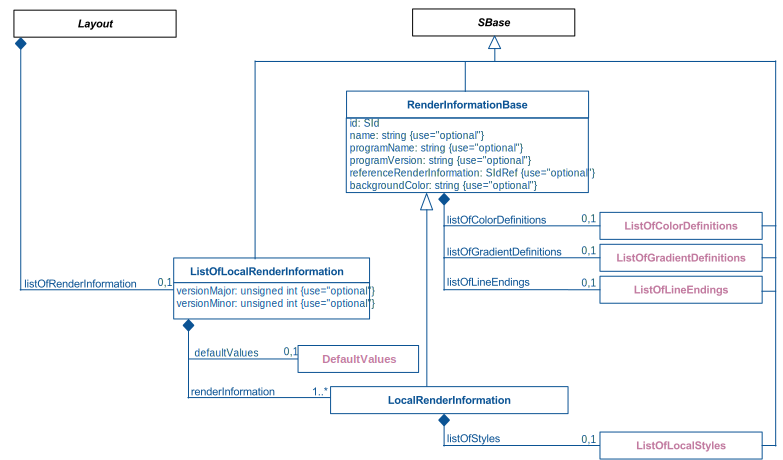
\includegraphics[width=\textwidth]{images/render-layout-uml}\\
  \caption{A UML representation of the extended \Layout class for the \RenderPackage. See \ref{conventions} for conventions related to this figure.}
  \label{fig:Render_uml}
\end{figure}

\begin{figure}[!h]
  \centering
  % Requires \usepackage{graphicx}
  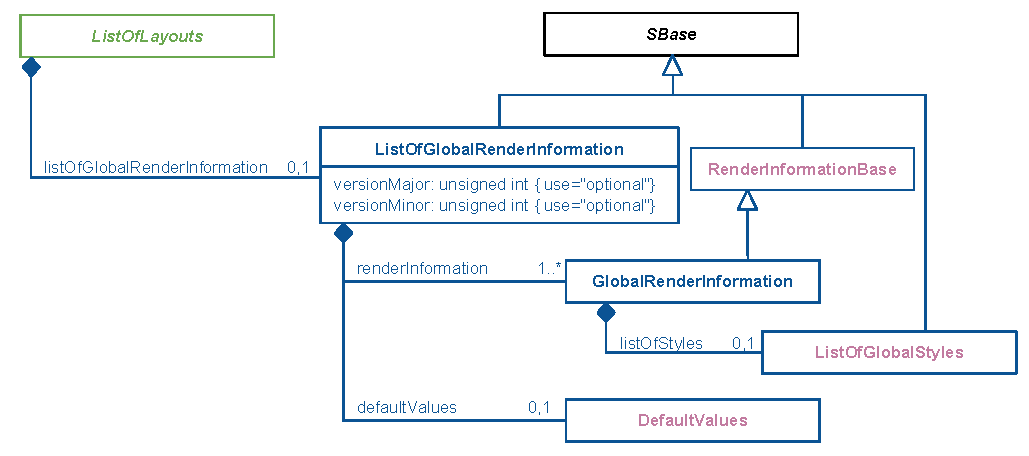
\includegraphics[width=\textwidth]{images/render-listoflayout-uml}\\
  \caption{A UML representation of the extended \ListOfLayouts object for the \RenderPackage.  See \ref{conventions} for conventions related to this figure. }
  \label{fig:lol_render_uml}
\end{figure}

It is important to note that each layout can have more than one 
set of local render information and that it is 
also possible to define more then one global style. Each style can also 
reference another style that complements it. This way the user can create 
styles that are based on other styles. In contrast to local styles, the global styles can not 
reference individual layout elements by an id, they can only define role based or 
type based styles.

%--------------------------------------------------------
\subsubsection{Uniqueness of ids}
\label{unique-id}

Since local and global render information objects can reference other render information objects, programs creating
render information need to make sure that all the ids are unique within the reference history. In other words, a 
render information object that references another render information object must make sure that none of its ids is equal
to an id in any of the directly or indirectly referenced render information objects. 

An exception to this rule is that a \ColorDefinition may have the same \token{id} as a \ColorDefinition in a referenced style. In this case interpreting programs can assume that this \ColorDefinition is supposed to override the \ColorDefinition with the
same \token{id} in the referenced render information object. Likewise it is also possible to override a \ColorDefinition with a  gradient ( that is either a \LinearGradient or a \RadialGradient) and vice versa. \LineEnding definitions on the other hand can only be replaced by other \LineEnding definitions.

%----------------------------------------------------------
\subsubsection{Default Values}
\label{defaultvalues-class}
Previously the render package specifed default values and inheritance in a similar fashion to the specification used by SVG. However, in order to comply with the \SBML 
development guidelines for Level~3 packages, we introduced a new class \DefaultValues to encode these values within the model. 
The \DefaultValues class can occur as a child of either the \ListOfGlobalRenderInformation or a 
\ListOfLocalRenderInformation. 

\begin{figure}[h!]
  \centering
  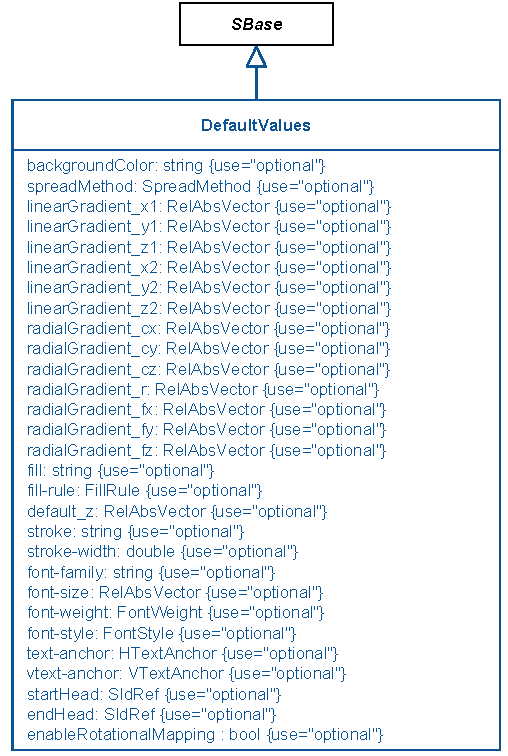
\includegraphics{images/render-default-values}\\
  \caption{A UML representation of the \DefaultValues class for the \RenderPackage.  See \ref{conventions} for conventions related to this figure. }
  \label{fig:default-values}
\end{figure}

The values from the \DefaultValues class are to be taken as 
default source for the values of any optional attribute that is not explicitly declared. An example on how to use the \DefaultValues 
class is below. For the meaning of the individual attributes, please see the 
corresponding sections later in this document. If an attribute has not been declared, either explicitly on an element or using the \DefaultValues class then software reading the XML may chose how they handle the attribute.

Note that the \DefaultValues associated with a \ListOfLocalRenderInformation will override \DefaultValues declared on the \ListOfGlobalRenderInformation.
\pagebreak
\exampleFile{examples/defaultValues.txt}


%----------------------------------------------------------
\subsection{Extended elements from the \LayoutPackage}


% ---------------------------------------------------------
\subsubsection{The extended \class{GraphicalObject} class}
\label{graphicalobject-class}

The \RenderPackage extends the \class{GraphicalObject} object from the \LayoutPackage with the
addition of
the \token{objectRole} attributes.

\paragraph{The \fixttspace\token{objectRole} attribute}


A \GraphicalObject has an optional attribute \token{objectRole} of type
\primtype{string}.  This attribute specifies with which \Style the object should be rendered. 
In the example below a \SpeciesGlyph is tagged with the role \val{SBO-0000285-clone}
later on a style in a \GlobalRenderInformation element includes that role in its 
\token{roleList} attribute and will be applied.

\exampleFile{examples/graphicalObjectExample.txt}


% ---------------------------------------------------------
\subsubsection{The extended \class{ListOfLayouts} class}
\label{listoflayouts-class}

The \RenderPackage extends the \class{ListOfLayouts} object from the \LayoutPackage with the
addition of an optional \ListOfGlobalRenderInformation object (\ref{fig:lol_render_uml}).

% ---------------------------------------------------------
\paragraph{The \class{ListOfGlobalRenderInformation} class}
\label{listofglobalrenderinformation-class}

The \ListOfGlobalRenderInformation object inherits the core attributes and subobjects from the
\class{SBase} class. It contains one or more objects of type
\GlobalRenderInformation.

In addition the \ListOfGlobalRenderInformation object has the optional attributes 
\token{versionMajor} and \token{versionMinor} as well as an optional \DefaultValues 
element that provides the default values for the \GlobalRenderInformation objects
contained in the list.

\paragraph{The \fixttspace\token{versionMajor} attribute}

A \ListOfGlobalRenderInformation has an optional attribute
\token{versionMajor} of type \primtype{unsigned integer} which specifies the major version of the render information.  Note this attribute is included to preserve backward compatibility with software using the \RenderPackage as a Level~2 annotation. If used it is recommended that the value is set to \val{1}.
 
\paragraph{The \fixttspace\token{versionMinor} attribute}

A \ListOfGlobalRenderInformation has an optional attribute
\token{versionMinor} of type \primtype{unsigned integer} which specifies the minor version of the render information.  Note this attribute is included to preserve backward compatibility with software using the \RenderPackage as a Level~2 annotation. If used, it is recommended that the value is set to \val{0}.
 

% ---------------------------------------------------------
\subsubsection{The extended \class{Layout} class}
\label{layout-class}

The \RenderPackage extends the \class{Layout} object from the \LayoutPackage with the addition
of an optional  \ListOfLocalRenderInformation object (\ref{fig:Render_uml}).

% ---------------------------------------------------------
\paragraph{The \class{ListOfLocalRenderInformation} class}
\label{listoflocalrenderinformation-class}

The \ListOfLocalRenderInformation object inherits the core attributes and subobjects from the \class{SBase}
class. It contains one or more objects of type \LocalRenderInformation.

In addition the \ListOfLocalRenderInformation object has the optional
attributes \token{versionMajor} and \token{versionMinor} as well as an optional
\DefaultValues element that provides the default values for the 
\LocalRenderInformation objects contained in the list.

\paragraph{The \fixttspace\token{versionMajor} attribute}

A \ListOfLocalRenderInformation has an optional attribute
\token{versionMajor} of type \primtype{unsigned integer} which specifies the major version of the render information.  Note this attribute is included to preserve backward compatibility with software using the \RenderPackage as a Level~2 annotation. If used it is recommended that the value is set to \val{1}.
 
\paragraph{The \fixttspace\token{versionMinor} attribute}

A \ListOfLocalRenderInformation has an optional attribute
\token{versionMinor} of type \primtype{unsigned integer} which specifies the minor version of the render information.  Note this attribute is included to preserve backward compatibility with software using the \RenderPackage as a Level~2 annotation. If used, it is recommended that the value is set to \val{0}.
 
%----------------------------------------------------------
%----------------------------------------------------------
\subsection{Render Information}
\label{renderinformation-class}
The render information classes hold all information about the rendering. The
information is stored between three classes: \RenderInformationBase, the base class with 
common features; \GlobalRenderInformation a class applying to types and roles of 
elements on a global level; and \LocalRenderInformation that provides additional information that can be applied to individual elements from the \LayoutPackage. These classes are illustrated in \ref{fig:Render_uml} and \ref{fig:lol_render_uml}.

% ---------------------------------------------------------
\subsubsection{The \class{RenderInformationBase} class}
\label{renderinformationbase-class}

The \RenderInformationBase class is an abstract class that holds all the 
information that is common to both local and global render 
information objects. It  derives from the \SBase class and thus
inherits any attributes and elements that are present on this class. In 
addition the \RenderInformationBase has the required attribute \token{id} and the 
optional attributes \token{name}, \token{programName}, \token{programVersion}, 
\token{referenceRenderInformation} and \token{backgroundColor}. Additionally it may
contain a \ListOfColorDefinitions, \ListOfGradientDefinitions and / or a \ListOfLineEndings. 
These lists are optional, however if present may not be empty. There may only be one 
of each of those lists. 

\paragraph{The \fixttspace\token{id} attribute}

A \RenderInformationBase has a required attribute \token{id} of type
\primtype{SId}. This \token{id} may be used to reference this \RenderInformation 
object from other elements within the \RenderPackage.

\paragraph{The \fixttspace\token{name} attribute}

A \RenderInformationBase has an optional attribute \token{name} of type
\primtype{string}. This \token{name} attribute can be used to give the object a 
more user friendly identifier.

\paragraph{The \fixttspace\token{programName} attribute}

A \RenderInformationBase has an optional attribute \token{programName}
of type \primtype{string} which can be used to store the name of the program 
that was used to create the render information.

\paragraph{The \fixttspace\token{programVersion} attribute}

A \RenderInformationBase has an optional attribute
\token{programVersion} of type \primtype{string} which can be used to store 
the version number of the program used to create the render information.

\paragraph{The \fixttspace\token{referenceRenderInformation} attribute}

A \RenderInformationBase has an optional attribute
\token{referenceRenderInformation} of type \primtype{SIdRef} which can be used to 
specify the \token{id} of another local or global render information object 
that complements the current render information object. A program reading and 
interpreting the render information can use this information to access another 
render information object, should the current object contain unsuitable information (i.e. information that the reading software cannot render). 

A \LocalRenderInformation object may reference any 
\GlobalRenderInformation object but may only reference \LocalRenderInformation objects defined within the same parent \class{Layout} object. 
A \GlobalRenderInformation object may only reference other \GlobalRenderInformation objects. Cyclical references are not allowed.


\paragraph{The \fixttspace\token{backgroundColor} attribute}

A \RenderInformationBase has an optional attribute
\token{backgroundColor} of type \colorString which defines the background 
color for rendering.

\paragraph{The \class{ListOfColorDefinitions} class}
\label{listofcolordefinitions-class}

The \ListOfColorDefinitions object
inherits the core attributes and subobjects from the \class{SBase}
class. It contains one or more objects of type \ColorDefinition which are used to predefine a set of colors to be referenced by \Styles. 

\paragraph{The \class{ListOfGradientDefinitions} class}
\label{listofgradientdefinitions-class}

The \ListOfGradientDefinitions object inherits the core attributes and subobjects from the \class{SBase}
class. It contains one or more objects of type \GradientBase which are used to define either \LinearGradient or \RadialGradient objects to be used in \Styles. 

\paragraph{The \class{ListOfLineEndings} class}
\label{listoflineendings-class}

The \ListOfLineEndings object
inherits the core attributes and subobjects from the \class{SBase}
class. It contains one or more objects of type \LineEnding which can be used to define a set of \LineEndings that can be applied to path objects.


% ---------------------------------------------------------
\subsubsection{The \class{LocalRenderInformation} class}
\label{localrenderinformation-class}
The \RenderInformation element of type \LocalRenderInformation is the primary 
container that holds the render information for a \class{Layout} instance. 


The \LocalRenderInformation object derives from the
\RenderInformationBase class and thus inherits any attributes and
elements that are present on this class.
A \LocalRenderInformation may contain exactly one element named \token{listOfStyles} 
of type \ListOfLocalStyles.

\paragraph{The \class{ListOfLocalStyles} class}
\label{listoflocalstyles-class}

The \ListOfLocalStyles object inherits
the core attributes and subobjects from the \class{SBase} class. It is optional but 
if present has to contain one or more objects of type \LocalStyle.


% ---------------------------------------------------------
\subsubsection{The \class{GlobalRenderInformation} class}
\label{globalrenderinformation-class}

Global render information is specified in a very similar way as local render information. The attributes and elements of \GlobalRenderInformation objects and 
\LocalRenderInformation objects are the same with the exception of the \token{listOfStyles} element. In the case of a \GlobalRenderInformation object the \token{listOfStyles} element is of type \ListOfGlobalStyles.

It should be noted that another difference between \GlobalRenderInformation and \LocalRenderInformation is the 
fact that \GlobalRenderInformation objects may only reference ids of other 
\GlobalRenderInformation objects in their \token{referenceRenderInformation} attribute. 

\paragraph{The \class{ListOfGlobalStyles} class}
\label{listofglobalstyles-class}

The \ListOfGlobalStyles object inherits
the core attributes and subobjects from the \class{SBase} class. It
contains one or more objects of type \GlobalStyle.

\vspace{0.25cm}
The following snippet shows the general outline of a \ListOfGlobalRenderInformation object:


{\footnotesize
\begin{example}
<layout:listOfLayouts>
   <render:listOfGlobalRenderInformation>
      <render:renderInformation render:id="FancyRenderer_GlobalDefault" 
                         render:name="default global style" 
                         render:programName="FancyRenderer" 
                         render:programVersion="0.1.1">
        <render:listOfColorDefinitions>
             ...
        </render:listOfColorDefinitions>
        <render:listOfGradientDefinitions>
             ...
        </render:listOfGradientDefinitions>
        <render:listOfLineEndings>
             ...
        </render:listOfLineEndings>
        <render:listOfStyles>
             ...
        </render:listOfStyles>
      </render:renderInformation>
   </render:listOfGlobalRenderInformation>
</layout:listOfLayouts>
\end{example}
}
%---------------------------------------------------------
%---------------------------------------------------------
\subsection{Styles}


\begin{figure}[h!]
  \centering
  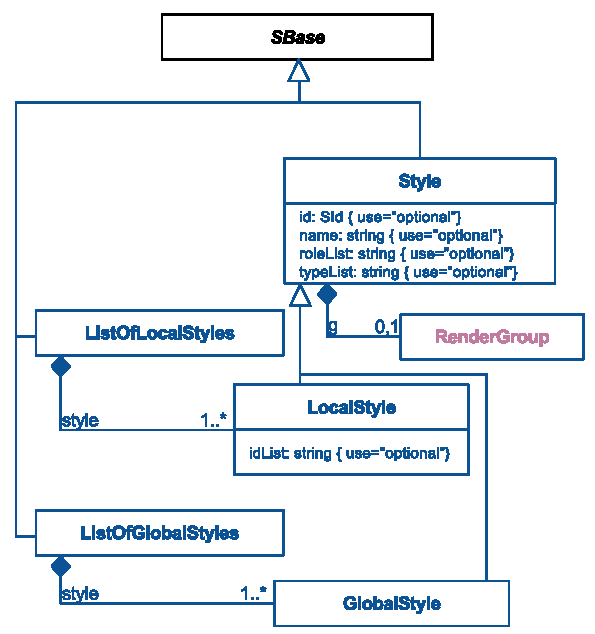
\includegraphics{images/render-style-uml}\\
  \caption{A UML representation of the \Style object for the \RenderPackage.
	See \ref{conventions} for conventions related to this figure. }
  \label{fig:style_render_uml}
\end{figure}
% ---------------------------------------------------------
\subsubsection{The \class{Style} class}
\label{style-class}

The \Style class that holds all the information that is common to both local and global styles (\ref{fig:style_render_uml}). The \Style object derives from the \SBase class and thus inherits any
attributes and elements that are present on this class.
A \Style element may contain exactly one \RenderGroup element.
In addition the \Style object has the optional attributes \token{id}, \token{name}, \token{roleList} and \token{typeList}.

The \RenderGroup element, \val{g}, is used to specify how the elements covered by this \Style object are to be rendered and is discussed fully in \ref{rendergroup-class}. 

\paragraph{The \fixttspace\token{id} attribute}

A \Style has an optional attribute \token{id} of type \primtype{SId} which can be used to uniquely identify this \Style object.

\paragraph{The \fixttspace\token{name} attribute}

A \Style has an optional attribute \token{name} of type
\primtype{string} which can be used to provide a more user friendly identifier.

\paragraph{The \fixttspace\token{roleList} attribute}

A \Style has an optional attribute \token{roleList} of type
\primtype{string}. The string value of the \token{roleList} attribute contains 
a space separated list of all the roles to which this \Style should be applied.

This attribute can be  used in conjunction with the \token{objectRole} attribute 
that is used to extend the \GraphicalObject class from the \LayoutPackage. If 
the string given as an \token{objectRole} value appears in the \token{roleList} 
attribute of some render information object, then that render information object
applies to the graphical object as shown in the snippet below. Note this 
relationship is only valid if there is no render information object that is more 
specific. For example another \LocalStyle could be defined with \token{idList} 
that references the \token{layout:id="go1"} explicitly, in which case that style 
would be  chosen. For more information see also \sec{style-res}. 

{\footnotesize
\begin{example}
<layout:layout>
   <layout:listOfAdditionalGraphicalObjects>
      <layout:graphicalObject layout:id="go1" render:objectRole="Parameter">
         ...
      </layout:graphicalObject>
   </layout:listOfAdditionalGraphicalObjects>
   <render:listOfLocalRenderInformation>
      <render:renderInformation render:id="FancyRenderer_GlobalDefault">
             ...
        <render:listOfStyles>
             <render:style render:id="style_1" render:roleList="Parameter">
                <g> ... </g>
             </render:style> 
        </render:listOfStyles>
      </render:renderInformation>
   </render:listOfLocalRenderInformation>
</layout:layout>
\end{example}
}


\paragraph{The \fixttspace\token{typeList} attribute}

A \Style has an optional attribute \token{typeList} of type
\primtype{string}. The string value of the \token{typeList} attributes contains 
a space separated list of one or more of the values from the \StyleType enumeration.
 The example snippet shows a particular style that is to be applied to 
both \class{SpeciesGlyph} and \class{SpeciesReferenceGlyph} objects from 
the \LayoutPackage.

\pagebreak
{\footnotesize
\begin{example}
<layout:listOfLayouts>
   <render:listOfGlobalRenderInformation>
      <render:renderInformation render:id="FancyRenderer_GlobalDefault">
             ...
        <render:listOfStyles>
             <render:style render:id="style_1" render:typeList="SPECIESGLYPH SPECIESREFERENCEGLYPH">
                <g> ... </g>
             </render:style> 
        </render:listOfStyles>
      </render:renderInformation>
   </render:listOfGlobalRenderInformation>
</layout:listOfLayouts>
\end{example}
}

% ---------------------------------------------------------
\subsubsection{The \class{GlobalStyle} class}
\label{globalstyle-class}

The \GlobalStyle object derives from the \Style class and thus inherits
any attributes and elements that are present on this class. The \GlobalStyle 
class is used for objects in the \ListOfGlobalStyles element of a 
\GlobalRenderInformation object.



% ---------------------------------------------------------
\subsubsection{The \class{LocalStyle} class}
\label{localstyle-class}

The \LocalStyle object derives from the \Style class and thus inherits
any attributes and elements that are present on this class. It is identical to 
the \GlobalStyle object but has an additional optional \token{idList} attribute.

The \LocalStyle class is used for objects in the \ListOfLocalStyles element of a 
\LocalRenderInformation object.

\paragraph{The \fixttspace\token{idList} attribute}

A \LocalStyle has an optional attribute \token{idList} of type
\primtype{string} which is a space separated list of ids of layout objects to 
which this \Style should be applied.


% ---------------------------------------------------------
%----------------------------------------------------------
\subsection{Colors and Gradients}

All \RenderInformation objects may contain a \ListOfColorDefinitions containing 
objects of type \ColorDefinition and a \ListOfGradientDefinitions containing 
objects of type \GradientBase. Gradients consist of continuously smooth color 
transitions along a vector from one color to another, possibly followed by 
additional transitions along the same vector to other colors. Here the \RenderPackage 
borrows heavily from the SVG specification. These are described in more detail in this section. 
 
\subsubsection{The \class{ColorDefinition} class}
\label{colordefinition-class}

\begin{figure}[h!]
  \centering
  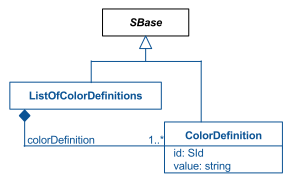
\includegraphics{images/render-color-definition-uml}\\
  \caption{A UML representation of the \ColorDefinition object for the \RenderPackage.  See \ref{conventions} for conventions related to this figure. }
  \label{fig:color_render_uml}
\end{figure}


The \ColorDefinition object derives from the \SBase class and thus
inherits any attributes and elements that are present on this class.
In addition the \ColorDefinition object has the optional attributes \token{id} and \token{value}.

\paragraph{The \fixttspace\token{id} attribute}

A \ColorDefinition has a required attribute \token{id} of type
\primtype{SId} which is used to give the \ColorDefinition an unique identifier within the \RenderInformation object.

\paragraph{The \fixttspace\token{value} attribute}

A \ColorDefinition has a required attribute \token{value} of type
\colorString. Instead of 
specifying a color value, the value \val{none} can be given which is equivalent to 
no drawing at all.

The example snippet defines a dark red color, with a red component of 0x20, green 
component of 0x00, and blue component of 0x00. Since it is not specifying the alpha 
component, it will have the value of 0xff. 

{\footnotesize
\begin{example}
<listOfColorDefinitions>
  <colorDefinition id="darkred" value="#200000" />
       ...
</listOfColorDefinitions>
\end{example}
}


% ---------------------------------------------------------
\subsubsection{The \class{GradientBase} class}
\label{gradientbase-class}

\begin{figure}[h!]
  \centering
  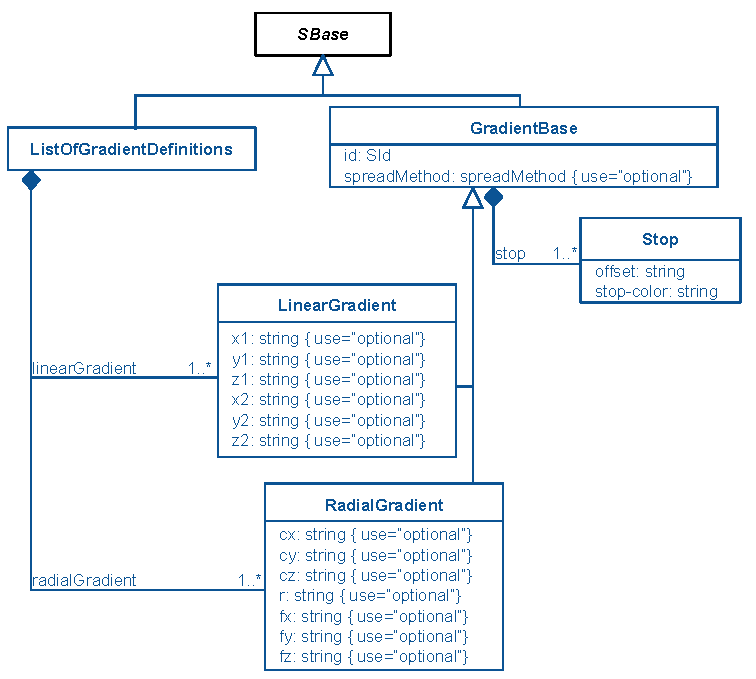
\includegraphics{images/render-gradient-definitions-uml}\\
  \caption{A UML representation of the gradient objects for the \RenderPackage.  See \ref{conventions} for conventions related to this figure. }
  \label{fig:gradient_render_uml}
\end{figure}


\GradientBase is an abstract class that holds all the information that is common to both \RadialGradient and \LinearGradient objects (\ref{fig:style_render_uml}).The \GradientBase object derives from the \SBase class and thus inherits
any attributes and elements that are present on this class.
A \GradientBase may contain one or more \GradientStop elements.
In addition the \GradientBase object has a required \token{id} attribute and an optional \token{spreadMethod} attribute.

\paragraph{The \fixttspace\token{id} attribute}

A \GradientBase has a required attribute \token{id} of type
\primtype{SId} which is used to uniquely identify or reference a gradient within an \RenderInformation object.

\paragraph{The \fixttspace\token{spreadMethod} attribute}

A \GradientBase has an optional attribute \token{spreadMethod} of type
\GradientSpreadMethod that specifies the method that is
used to continue the gradient pattern if the vector points do not span the whole
bounding box of the object to which the gradient is applied. 

% ---------------------------------------------------------
%\paragraph{The \GradientStop elements}
%\label{listofgradientstops-class}
%
%The \ListOfGradientStops object 
%inherits the core attributes and subobjects from the \class{SBase}
%class. It contains one or more objects of type \GradientStop.
%

% ---------------------------------------------------------
\subsubsection{The \class{GradientStop} class}
\label{gradientstop-class}

As the name suggests the \GradientStop object is used to define "gradient stops" 
which are used in line with the SVG specification.
The \GradientStop object derives from the \SBase class and thus inherits
any attributes and elements that are present on this class.
In addition the \GradientStop object has the required attributes \token{offset}
and \token{stop-color}. Note, unlike most SBML elements, the XML element name does not match the class name. The name of a \GradientStop element is \val{stop} to preserve backward compatibility with render used in Level~2 annotations.

\paragraph{The \fixttspace\token{offset} attribute}

A \GradientStop has a required attribute \token{offset} of type
\RelAbsVector which represents the relative distance from the starting point of 
the gradient. Depending on the type of gradient, this is either the point 
defined by the \token{x1},\token{y1} and \token{z1} attributes (\LinearGradient) 
or the \token{fx}, \token{fy} and \token{fz} attributes (\RadialGradient). 
This value is given as a positive percentage value. Note when using 2 dimensions the z values \token{z1} or \token{fz} are not required.

\paragraph{The \fixttspace\token{stop-color} attribute}

A \GradientStop has a required attribute \token{stop-color} of type
\primtype{string} which defines the color for the given gradient stop. The
attributes value can either be given as a hexadecimal color value (i.e. type \colorString) or as the id
of a \ColorDefinition object from the \ListOfColorDefinitions(i.e. type \primtype{SIdRef}).    

The \token{id} of a \ColorDefinition specifing \val{none} as its \token{value} cannot be used as a \token{stop-color}. It is also considered an error to specify the id of another gradient as the value of a \token{stop-color} attribute.
In the case where the two points that define the gradient vector are identical, the area
is to be painted with a single color taken from the last gradient stop element.

There are a few rules that need to be considered when working with gradient stops.
%Basically these rules are the same as defined by the SVG specification.

\begin{enumerate}
\item{The offset value of a gradient stop should be between 0\% and 100\%.}
% If the offset lies outside of this value, the value is adjusted to be either 0\% if the given value is smaller than 0\% or to 100\% if the value is greater than 100\%.}
\item{The absolute part in any offset value is ignored, meaning it is considered to be 0.0 even if specified otherwise in a gradient stop.}
\item{The offset of any gradient stop should to be greater than the offset of the preceding gradient stop.}
%\item{If two gradient stops have the same offset value, the last gradient stop with this offset value determines the color at this point in the gradient.}
\end{enumerate}

Historically the render specification applied the same rules as the SVG specification. The above is a simplification of these rules but users should be aware that existing implementations and models apply the following defaults when encountering models that do not comply with the rules above. 

\begin{itemize}
\item{An offset that is less that 0\% is adjusted to be 0\%.}
\item{An offset that is greater than 100\% is adjusted to be 100\%.}
\item{If an offset has a value less than that of the preceding stop, the offset is adjusted to have the same value as the preceding stop.}
\item{If there are multiple stops with the same offset, the color used is that of the final stop with the duplicate offset value.}
\end{itemize}
% ---------------------------------------------------------
\subsubsection{The \class{LinearGradient} class}
\label{lineargradient-class}

The \LinearGradient provides the vector points that define the start and end points to which the \GradientStop elements should be mapped.

The \LinearGradient object derives from the \GradientBase class and thus
inherits any attributes and elements that are present on this class.
In addition the \LinearGradient object has the attributes  \token{x1}, \token{y1},
\token{z1}, \token{x2}, \token{y2} and \token{z2}. As the names suggest these represent the x, y and z coordinates in a three dimensional Cartesian system. If only the x and y attributes are used a two dimensional viewport is assumed.

Note that these attributes are all considered optional. This is to preserve compatibility with the historical render specification that used default values (see \sect{defaultvalues-class}. The current recommendation is that the \token{x} and \token{y} values are considered required.

Since the value for the vector can be specified as an absolute value or one that is relative to the current viewport these attributes all have values of type \RelAbsVector.

\paragraph{The \fixttspace\token{x1}, \fixttspace\token{y1} and \fixttspace\token{z1} attributes}

The attributes \token{x1}, \token{y1} and \token{z1} define the start point of the gradient in either two (\token{z1} undefined) or three dimensions.

\paragraph{The \fixttspace\token{x2}, \fixttspace\token{y2} and \fixttspace\token{z2} attributes}

The attributes \token{x2}, \token{y2} and \token{z2} define the end point of the gradient in either two (\token{z2} undefined) or three dimensions.



{
  {\bf
Example of specifying the \LinearGradient shown in \ref{fig:lingrad}:
}
}
{\footnotesize
\begin{example}
<listOfGradientDefinitions>
  <linearGradient x1="12.5%" y1="25%" x2="87.5%" y2="75%">
    <stop offset="5%" stop-color="#000F60" />
    <stop offset="95%" stop-color="#000FF6" />
  </linearGradient>
        ...
</listOfGradientDefinitions>
\end{example}
}

\begin{figure}[h!]
  \centering
  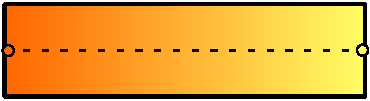
\includegraphics{figures/lingrad01.pdf}\\
  \caption{Example of a \LinearGradient}
  \label{fig:lingrad}
\end{figure}


% ---------------------------------------------------------
\subsubsection{The \class{RadialGradient} class}
\label{radialgradient-class}


The \RadialGradient object derives from the \GradientBase class and thus
inherits any attributes and elements that are present on this class.
In addition the \RadialGradient object has seven attributes (each of type \RelAbsVector) that are used to define the center, radius and focal point of the gradient.



\paragraph{The \fixttspace\token{cx}, \fixttspace\token{cy} and \fixttspace\token{cz} attributes}

The attributes \token{cx}, \token{cy} and \token{cz} define the center of the gradient as a point in either two (\token{cz} undefined) or three dimensions.


\paragraph{The \fixttspace\token{r} attribute}

The attribute \token{r} defines the radius of the gradient and must be positive. If the radius is given in relative values, the relation is to the width as well as the height. This means that 
if the width of the bounding box and the height of the bounding box are not equal, \token{cx},\token{cy},\token{cz}
and \token{r} don't actually specify a circle, but an ellipse.

\paragraph{The \fixttspace\token{fx}, \fixttspace\token{fy} and \fixttspace\token{fz} attributes}

The attributes \token{fx}, \token{fy} and \token{fz} define the focal point of the gradient as a point in either two (\token{fz} undefined) or three dimensions. The gradient is drawn such that this point is mapped to the 0\% \GradientStop. If one of these attributes is left undeclared it is considered to be equal to the corresponding coordinate of the center point. If the focal point lies outside 
the circle, the focal point is considered to be located on the intersection of the the line from the center
point to the focal point and the sphere determined by the center point and the radius.

Note that these attributes are all considered optional. This is to preserve compatibility with the historical render specification that used default values (see \sec{defaultvalues-class}. The current recommendation is that the \token{x}, \token{y} and \token{r} values are considered required.

  {\bf
Example of specifying the \RadialGradient shown in \ref{fig:radgrad}:
}

{\footnotesize
\begin{example}
<listOfGradientDefinitions>
  <radialGradient cx="50%" cy="50%" r="300" fx="50%" fy="50%">
    <stop offset="0%" stop-color="#FF0000" />
    <stop offset="50%" stop-color="#0000FF" />
    <stop offset="100%" stop-color="#FF0000" />
  </radialGradient>
       ...
</listOfGradientDefinitions>
\end{example}
}

\begin{figure}[h!]
  \centering
  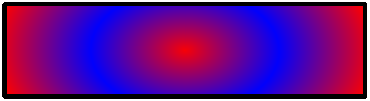
\includegraphics{figures/radgrad01.pdf}\\
  \caption{Example of a \RadialGradient}
  \label{fig:radgrad}
\end{figure}



%\begin{figure}[h!]
%  \centering
%  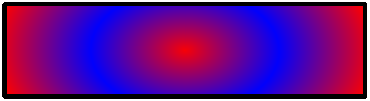
\includegraphics[scale=0.5]{figures/radgrad01.pdf}\\
%  \caption{Example of a \RadialGradient}
%  \label{fig:radgrad}
%\end{figure}



%--------------------------------------------------------
%---------------------------------------------------------
\subsection{Transformation}

In order to be able to display text that is not aligned horizontally or 
vertically or to effectively compose groups of objects from primitives, 
transformations like rotation, translation and scaling are needed. SVG, among 
other options, allows the user to specify a 3x3 matrix transformation matrix: 

\hspace*{0.4cm}
\begin{center}
\begin{math}\left[ \begin{array}{ccc} a & c & e \\ b & d & f \\ 0 & 0 & 1\end{array}\right]\end{math}
\end{center}
\hspace*{0.4cm}

Since the last row of the matrix is always 0 0 1, the matrix is specified as a 
six value vector. In the render extension each group or graphical 
primitive is derived from the class \TransformationTwoD and can have a \token{transform} attribute just as in SVG.

\begin{figure}[!h]
  \centering
  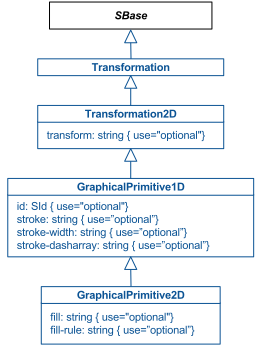
\includegraphics{images/render-base-classes-uml}\\
  \caption{A UML representation of the base graphical primitive classes for the \RenderPackage.  See \ref{conventions} for conventions related to this figure. }
  \label{fig:base_render_uml}
\end{figure}


% ---------------------------------------------------------
\subsubsection{The \class{Transformation} class}
\label{transformation-class}

The \Transformation class is a common base class for all elements that can be drawn.
Since both the \LayoutPackage and the \RenderPackage are currently limited to two dimensions, this class is only used as a base class for \TransformationTwoD and we leave the complete specification of this class for a future version of this document.


The \Transformation object derives from the \SBase class and thus
inherits any attributes and elements that are present on this class.
In addition the \Transformation object has the required \token{transform} attribute.

\paragraph{The \fixttspace\token{transform} attribute}

A \Transformation has a required attribute \token{transform} of type \doubleArray. This specifies an affine transformation matrix in three dimensions in which case the array must consist of exactly 12 values.

% ---------------------------------------------------------
\subsubsection{The \class{Transformation2D} class}
\label{transformationtwod-class}

Since the current render information specification only defines two dimensional objects, we derive a second class called \TransformationTwoD from \Transformation. As illustrated in \ref{fig:base_render_uml} the class \TransformationTwoD serves as the base class for all drawable 1D and 2D objects.

\paragraph{The \fixttspace\token{transform} attribute}

The \TransformationTwoD class restricts the transformation matrix to specify the six values of a 2D affine transformation. Thus the \token{transform} attribute consists of \doubleArray with exactly 6 values of type \primtype{double}. Thus the allowed 
value for the attribute has the form: "\token{a, b, c, d, e, f}"

The values for \token{a},\token{b},\token{c},\token{d},\token{e} and \token{f} depend on the transformation operation components and the order in which those transformation components are executed.

There are four basic transformation operations that can be combined in a affine transformation matrix.  Details of these are given in \apdx{apdx-transformations}.

All objects that are derived from \TransformationTwoD can have a transformation, this includes group elements. In contrast to other attributes on groups and children of groups, the transformation is not overwritten if it is specified in a child, but rather all transformations that are defined in an object hierarchy accumulate. Thus when a group specifies a transformation and a child of the group also sets a transformation, the transformation for the child has to be applied to the child only and the transformation that is set on the group has to be applied to the whole group, i.e. to all children of the group.

%--------------------------------------------------------
%--------------------------------------------------------
\subsection{GraphicalPrimitives}

The graphical primitives polygons, rectangles and ellipses are based on the 
corresponding elements from SVG. For lines, arcs and general path primitives, we 
introduce the \RenderCurve element which differs slightly from the \LayoutPackage \class{Curve}. 
Whereas \class{Point} objects in the \LayoutPackage could only contain 
absolute values for their coordinates, \RenderPoint objects in the \RenderPackage 
can contain relative coordinate values.  Two primitive abstract classes are defined to specify the common properties of 1D and 2D shapes.


% ---------------------------------------------------------
\subsubsection{The \class{GraphicalPrimitive1D} class}
\label{graphicalprimitiveoned-class}

The \GraphicalPrimitiveOneD object derives from the \TransformationTwoD
class and thus inherits any attributes and elements that are present on
this class (\ref{fig:base_render_uml}).
In addition the \GraphicalPrimitiveOneD object has the optional \token{id}, \token{stroke}, \token{stroke-width} and \token{stroke-dasharray} attributes.

\paragraph{The \fixttspace\token{id} attribute}

A \GraphicalPrimitiveOneD has an optional attribute \token{id} of type
\primtype{SId} which can be used to uniquely identify the object.

\paragraph{The \fixttspace\token{stroke} attribute}

A \GraphicalPrimitiveOneD has an optional attribute \token{stroke} of
type \primtype{string}. This is used to specify the color of the stroke that is used to draw the curve 
or the outline of geometric shapes. This \token{stroke}
attribute can either hold a color value or it can hold the id of a predefined
\ColorDefinition object.

\paragraph{The \fixttspace\token{stroke-width} attribute}

A \GraphicalPrimitiveOneD has an optional attribute \token{stroke-width}
of type \primtype{double} which specifies the width of the stroke to be used.

\paragraph{The \fixttspace\token{stroke-dasharray} attribute}

A \GraphicalPrimitiveOneD has an optional attribute
\token{stroke-dasharray} consisting of an array of values of type \\ \primtype{unsigned
integer}. This list specifies the lengths of dashes and 
gaps that are used to draw the line. The individual numbers in the list are separated by commas. 
For example,  "5,10" would mean to draw 5 points, make a 10 point gap, draw 5 points etc. If the pattern is to start with a gap, the first number has to be 0.

It should be noted that if a style defines a stroke dasharray and this style is applied to a \class{Curve} from the \LayoutPackage, one has to watch out for the fact that the layout curves may contain breaks (if the end point of segment n is not identical to the starting point of segment n+1). In this case each of the unbroken line stretches is considered a separate curve object and the line stippling is applied to each curve. That means the line stippling is not continuously applied through the gap, but it starts again after the gap.


% ---------------------------------------------------------
\subsubsection{The \class{GraphicalPrimitive2D} class}
\label{graphicalprimitivetwod-class}

The \GraphicalPrimitiveTwoD object derives from the
\GraphicalPrimitiveOneD class and thus inherits any attributes and
elements that are present on this class (\ref{fig:base_render_uml}).
In addition the \GraphicalPrimitiveTwoD object has the optional \token{fill} and \token{fill-rule} attributes.

\paragraph{The \fixttspace\token{fill} attribute}

A \GraphicalPrimitiveTwoD has an optional attribute \token{fill} of type
\primtype{string} which specifies 
the fill style of the object. The fill style can either be a hexadecimal
color value, the id of a \ColorDefinition object or the id of a \GradientBase
object. 
Instead of a color or gradient id, \val{none} can be specified
 which means that the object is unfilled.


\paragraph{The \fixttspace\token{fill-rule} attribute}

A \GraphicalPrimitiveTwoD has an optional attribute \token{fill-rule} of
type \FillRule that can be used to specify how the shape should be filled. 

Currently the \token{fill-rule} attribute is only useful for polygons. No other shapes have alternating areas.

% ---------------------------------------------------------
\subsubsection{The \class{RenderCurve} class}
\label{rendercurve-class}
\begin{figure}[!h]
  \centering
  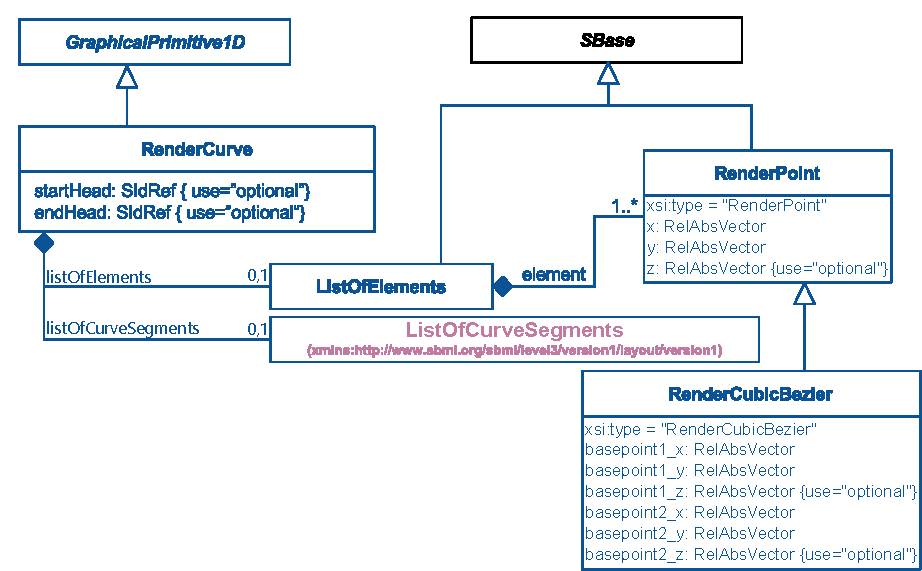
\includegraphics{images/render-curve-uml}\\
  \caption{A UML representation of the \RenderCurve classes for the \RenderPackage.  See \ref{conventions} for conventions related to this figure. }
  \label{fig:curve_render_uml}
\end{figure}

Simple lines and complex curves are represented by a \RenderCurve element. 

The \RenderCurve object derives from the \GraphicalPrimitiveOneD class (see \ref{fig:curve_render_uml})
and thus inherits any attributes and elements that are present on this
class.
A \RenderCurve contains at most one \ListOfElements element and at most one \class{ListOfCurveSegments} from the \LayoutPackage.
In addition the \RenderCurve object has the optional attributes \token{startHead} and \token{endHead}.

\paragraph{The \fixttspace\token{startHead} attribute}

A \RenderCurve has an optional attribute \token{startHead} of type
\primtype{SIdRef} and points to the \LineEnding that should be applied to the start of the path.

\paragraph{The \fixttspace\token{endHead} attribute}

A \RenderCurve has an optional attribute \token{endHead} of type
\primtype{SIdRef} and points to the \LineEnding that should be applied to the end of the path.

% ---------------------------------------------------------
\paragraph{The \class{ListOfElements} class}
\label{listofelements-class}

The \ListOfElements object inherits
the core attributes and subobjects from the \class{SBase} class. It
contains one or more objects of type \RenderPoint or of the derived type \RenderCubicBezier. 
The only restriction is that the first element must be a \RenderPoint.

Thus the first point specifies the start point of the curve. If the next element 
is another \RenderPoint, we have a straight line segment, going from the start point 
to the second point. Should the second point be a \RenderCubicBezier a cubic bezier curve 
will be added from the start point with its values. Thus the \ListOfElements holds a concise
definition of the curve specifying start and end points for all line segments. 

\paragraph{The \class{ListOfCurveSegments}}

The \LayoutPackage defines a similar \class{Curve} that has identical specification except it is restricted to using absolute values.  The classes involved have thus been redefined for the \RenderPackage which facilitates the use of relative values. However it is perfectly valid to use the \class{ListOfLineSegments} object from the \LayoutPackage either in place of the \ListOfElements or in addition to it. 

The example in \sec{rendercubicbezier-class} illustrates both the \ListOfElements and \class{ListOfCurveSegments} objects.

% ---------------------------------------------------------
\subsubsection{The \class{RenderPoint} class}
\label{renderpoint-class}

\RenderPoint objects are used to 
specify the individual curve segments.

The \RenderPoint object derives from the \SBase class and thus inherits
any attributes and elements that are present on this class.
In addition the \RenderPoint object has the required attributes \token{x} and \token{y} and the optional attribute \token{z}. It also has the required attribute \token{type} from the \val{xsi} namespaces.

\paragraph{The \fixttspace\token{x}, \fixttspace\token{y} and \fixttspace\token{z} attributes}

These three attributes are used to specify the coordinates of a  \RenderPoint in two (missing \token{z}) or three dimensions. They are of type \RelAbsVector and can thus specify a coordinate as either an absolute or relative value. The coordinate
values are always with respect to the bounding box of the layout object to which the
render information applies.

\paragraph{The \fixttspace\token{xsi:type} attribute}

For a \RenderPoint object this attribute will always have the value \val{RenderPoint}.


% ---------------------------------------------------------
\subsubsection{The \class{RenderCubicBezier} class}
\label{rendercubicbezier-class}


The \RenderCubicBezier object derives from the \RenderPoint class and
thus inherits any attributes and elements that are present on this
class.
In addition the \RenderCubicBezier object has the required attributes \token{basepoint1\_x}, \token{basepoint1\_y}, \token{basepoint2\_x} and \token{basepoint2\_y}. It also has the optional attributes \token{basepoint1\_z} and \\ \token{basepoint2\_z}.

\paragraph{The \fixttspace\token{basepoint1\_x}, \fixttspace\token{basepoint1\_y} and \fixttspace\token{basepoint1\_z} attributes}

These three attributes are used to specify the coordinates of the first basepoint of a \RenderCubicBezier in two (missing \token{basepoint1\_z}) or three dimensions. They are of type \RelAbsVector and can thus specify a coordinate as either an absolute or relative value. The coordinate
values are always with respect to the bounding box of the layout object to which the
render information applies.


\paragraph{The \fixttspace\token{basepoint2\_x}, \fixttspace\token{basepoint2\_y} and \fixttspace\token{basepoint2\_z} attributes}

These three attributes are used to specify the coordinates of the second basepoint of a \RenderCubicBezier in two (missing \token{basepoint2\_z}) or three dimensions. They are of type \RelAbsVector and can thus specify a coordinate as either an absolute or relative value. The coordinate
values are always with respect to the bounding box of the layout object to which the
render information applies.

\paragraph{The \fixttspace\token{xsi:type} attribute}

For a \RenderCubicBezier object this attribute will always have the value \val{RenderCubicBezier}.



The example snippet illustrates the definition of a \RenderCurve with two line segments 
that are to be painted using a black stroke with width 2.0.
The first line segment is a straight segment going from the objects left middle (0\%, 50\%) 
to the right middle(100\%, 50\%). The second segment represents a cubic bezier, that 
continues from the right middle(100\%, 50\%) back to the left middle(0\%, 50\%) with 
two control points at (50\%, 90\%).  The equivalent curve defined using the \class{ListOfLineSegments} from the \LayoutPackage is also included (assuming a $100 x 100$ square object).


{\footnotesize
\begin{example}
<render:g ...>

  <!-- the curve is defined in the render namespace -->
  <render:curve render:stroke-width="2.0" render:stroke="#000000" >

    <!-- using the listOfElements from the render namespace -->
    <render:listOfElements>
      <!-- define the first point -->
      <render:element xsi:type="RenderPoint" render:x="0%" render:y="50%" />

      <!-- The next item starts at the previous point -->
      <!-- It is also a point so draw a straight line from the start point to here -->
      <render:element xsi:type="RenderPoint" render:x="100%" render:y="50%" />

      <!-- The next item starts at the previous point -->
      <!-- It is a cubic bezier so draw a curve using the basepoints from the start point to here -->
      <render:element xsi:type="RenderCubicBezier" render:x="0%" render:y="50%"
              render:basepoint1\_x="50%" render:basepoint1\_y="90%"
              render:basepoint2\_x="50%" render:basepoint2\_y="90%" />
    </render:listOfElements>

    <!-- using the listOfCurveSegments from the layout namespace -->
    <layout:listOfCurveSegments>

      <!-- the first segment is a line from start to end point
      <layout:curveSegment xsi:type="LineSegment">
        <layout:start layout:x="0" layout:y="50" />
        <layout:end layout:x="100" layout:y="50"/>
      </layout:curveSegment>

      <!-- the second segment is a curve from start to end with given basepoints -->
      <layout:curveSegment xsi:type="CubicBezier">
        <layout:start layout:x="100" layout:y="50" />
        <layout:end layout:x="0" layout:y="50"/>
        <layout:basePoint1 layout:x="50" layout:y="90"/>
        <layout:basePoint2 layout:x="50" layout:y="90"/>
      </layout:curveSegment>
    </layout:listOfCurveSegments>
  
  </render:curve>
  ...
</render:g>
\end{example}
} 

%---------------------------------------------------------
%---------------------------------------------------------
\subsection{Geometric Shapes}
\label{shapes}

This section details the classes of geometric objects that can be defined using 
the transformations and graphical primitives described (see \ref{fig:group_render_uml}).

\begin{figure}[!htp]
  \centering
  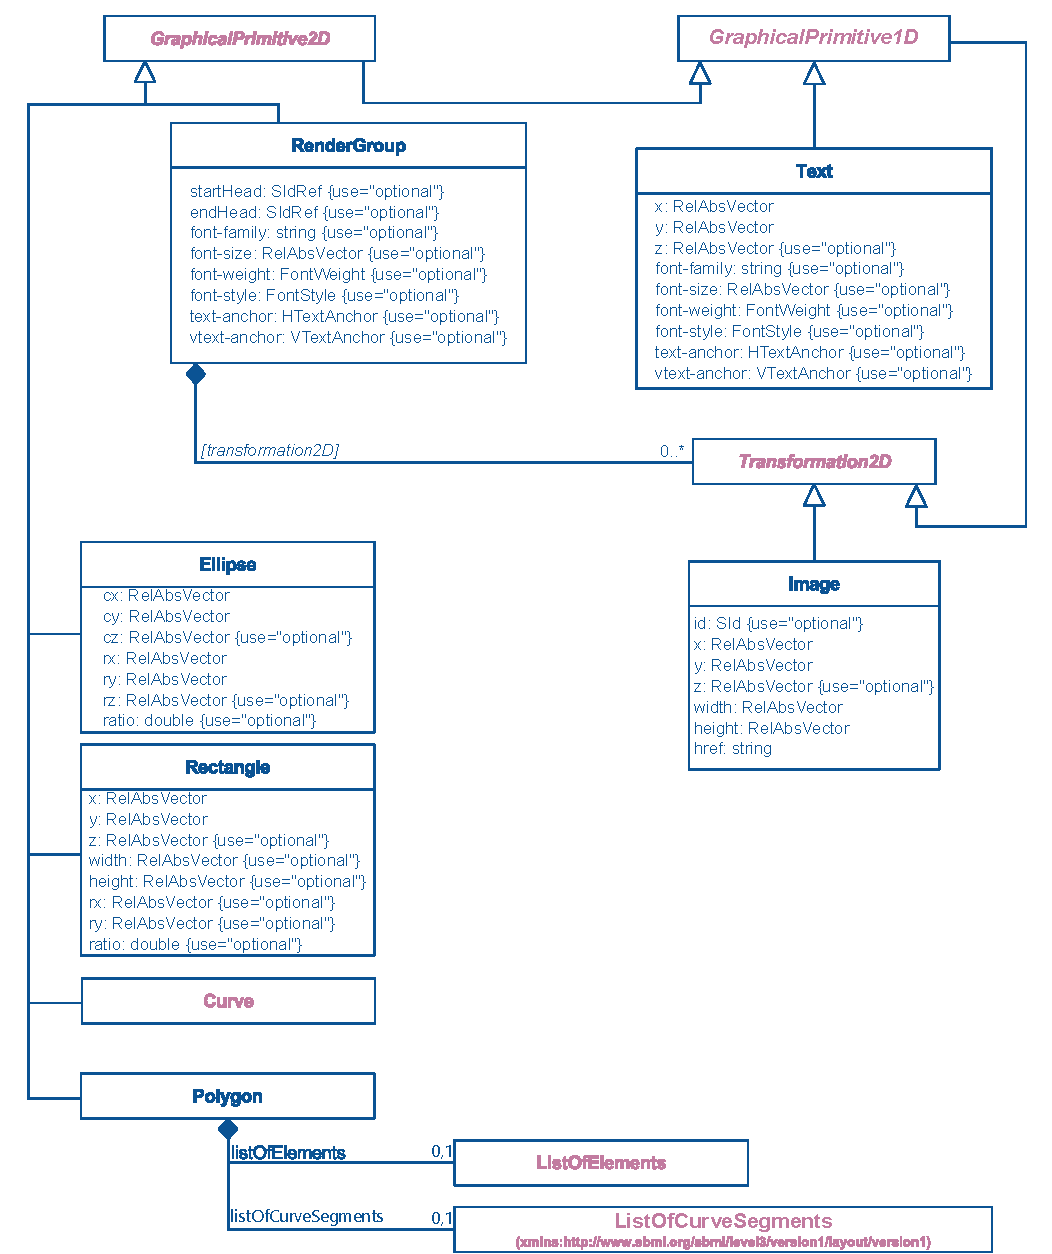
\includegraphics{images/render-group-uml}\\
  \caption{A UML representation of the graphical primitive classes for the \RenderPackage.  See \ref{conventions} for conventions related to this figure. }
  \label{fig:group_render_uml}
\end{figure}
\pagebreak


% ---------------------------------------------------------
\subsubsection{The \class{Polygon} class}
\label{polygon-class}

A \Polygon object is made up of a \texttt{polygon} element which contains at most one 
\ListOfElements and/or one \class{ListOf\-Curve\-Segments} used to define the edges of the polygon.

The major difference to the \RenderCurve 
object is that the object is always closed. 
That is, the last point of the curve is connected to the first.
Therefore, the polygon can have a fill style 
that determines how the inside of the polygon is to be rendered.

The example snippet shows the render specification of a \Polygon and of an unclosed path. It uses a 
black pen with width 3, and a red fill brush. \ref{PathVsPolygon} illustrates these shapes (without the red fill!).

{\footnotesize
\begin{example}
<g ...>
   <!-- define a path with three points -->
   <curve stroke="#000000" stroke-width="3">
     <listOfElements>
       <element xsi:type="RenderPoint" x="0%" y="0%"/>
       <element xsi:type="RenderPoint" x="100%" y="0%"/>
       <element xsi:type="RenderPoint" x="0%" y="100%"/>
     </listOfElements>
   </curve>

   <!-- the same points defined as a polygon
          so the last point draws a line to the first point -->
   <polygon stroke="#000000" stroke-width="3" fill="#FF0000">
     <listOfElements>
       <element xsi:type="RenderPoint" x="0%" y="0%"/>
       <element xsi:type="RenderPoint" x="100%" y="0%"/>
       <element xsi:type="RenderPoint" x="0%" y="100%"/>
     </listOfElements>
   </polygon>
</g>
\end{example}
}

\begin{figure}[!h]
\begin{center}
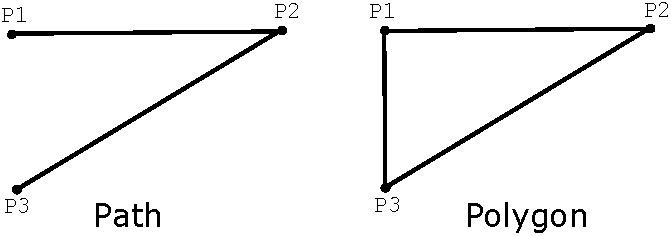
\includegraphics{figures/PathVsPolygon.pdf}
\end{center}
\caption{Rendering of a Path vs. rendering of a Polygon with the same base points}
\label{PathVsPolygon}
\end{figure}



% ---------------------------------------------------------
\subsubsection{The \class{Rectangle} class}
\label{renderrectangle-class}

The \RenderRectangle object was taken from the SVG specification and allows the 
definition of 
rectangles with or without rounded edges. 

The \RenderRectangle object derives from the \GraphicalPrimitiveTwoD
class and thus inherits any attributes and elements that are present on
this class.
In addition the \RenderRectangle object has the required attributes \token{x}, 
\token{y}, \token{height}, and \token{width} and the optional attributes 
\token{z}, \token{rx}, \token{ry} and \token{ratio}.

\paragraph{The \fixttspace\token{x}, \fixttspace\token{y} and \fixttspace\token{z}  attributes}

These attributes are of type
\RelAbsVector and specify its position within the 
bounding box of the enclosing layout object.

\paragraph{The \fixttspace\token{width} and \fixttspace\token{height} attribute}

These attributes are of type
\RelAbsVector and specify the width and height of the rectangle, 
either in absolute values or as a percentage of the width and height of the 
enclosing bounding box. 

\paragraph{The \fixttspace\token{rx} and \fixttspace\token{ry} attributes}

These attributes are of type
\RelAbsVector and specify the radius of the corner curvature. If only \token{rx}
or \token{ry} is specified, the other is presumed to have the same value as the 
one given. If no values are supplied this means that the edges are not rounded.
The relative values in rx and ry are in relation to the width and the height of
 the rectangle respectively. So a value of $10\%$ for rx means the radius of 
the corner is $10\%$ of the width of the rectangle. 


\paragraph{The \fixttspace\token{ratio} attribute}
If the optional \token{ratio} attribute of \primtype{double} is set, the biggest 
rectangle with the desired ratio of width to height is to be drawn centered in the 
objects bounding box. Using this approach makes it possible to always encode a 
square (by specifying \token{ratio="1"}), even if used with relative radii and a rectangular bounding box. 


% ---------------------------------------------------------
\subsubsection{The \class{Ellipse} class}
\label{renderellipse-class}


The \RenderEllipse object derives from the \GraphicalPrimitiveTwoD class
and thus inherits any attributes and elements that are present on this
class.
In addition the \RenderEllipse object has the required attributes \token{cx}, 
\token{cy} and \token{rx} and the optional attributes \token{ry}, \token{cz} and \token{ratio}.

\paragraph{The \fixttspace\token{cx}, \fixttspace\token{cy} and \fixttspace\token{cz}  attributes}

These attributes are of type
\RelAbsVector and specify the center of the ellipse.

\paragraph{The \fixttspace\token{rx} and \fixttspace\token{ry} attribute}

These attributes are of type
\RelAbsVector and specify the radius of the ellipse along the x-axis and y-axis 
respectively. If only one value is specified the other is assumed to have the same value. 

Circles are a special case where the \token{rx} and \token{ry} attributes have the same value. However, 
a circle will only be encoded if either the radii are specified absolutely, or if the bounding box is square. 
To encode circles for arbitrary bounding boxes and relative positioning please see the \token{ratio} 
attribute below.

\paragraph{The \fixttspace\token{ratio} attribute}
If the optional \token{ratio} attribute of \primtype{double} is set, the biggest 
ellipse with the desired ratio of width to height is to be drawn centered in the 
objects bounding box. Using this approach makes it possible to always encode a 
circle (by specifying \token{ratio="1"}), even if used with relative radii and a
rectangular bounding box. 

% ---------------------------------------------------------
\subsubsection{The \class{Text} class}
\label{text-class}

In order to draw text, we use the \token{text} element from SVG with slight 
modifications. For reasons of simplicity, we limit the display of text to normal 
text. Outlined or filled-outlined text are not supported.

Since we have a right handed coordinate system, the positive y axis normally 
faces downward on the screen if the positive z-axis goes into the screen. This 
means that text actually has to be renderer with the top towards lower y-values.


The \Text object derives from the \GraphicalPrimitiveOneD class and thus
inherits any attributes and elements that are present on this class.
In addition the \Text object has the required attributes \token{x} and \token{y} 
and the optional attributes \token{z}, \token{font-size}, \token{font-family}, 
\token{font-weight}, \token{font-style}, \token{text-anchor} and 
\token{vtext-anchor}.

\paragraph{The \fixttspace\token{x} attribute}

The \token{x} attribute is of type
\RelAbsVector and specifies the position of the horizontal text anchor.

\paragraph{The \fixttspace\token{y} attribute}

The \token{y} attribute is of type
\RelAbsVector and specifies the position of the vertical text anchor.

\paragraph{The \fixttspace\token{z} attribute}

The \token{z} attribute is of type
\RelAbsVector and directly specifies the depth value of the text element since 
there is no alignment attribute for text in the third dimension.

\paragraph{The \fixttspace\token{font-size} attribute}

A \Text has an optional attribute \token{font-size} of type \RelAbsVector which 
must have a positive value. In the case of a relative value it specifies a 
percentage of the height of the corresponding object. Combinations of relative 
and absolute values are not allowed.


\paragraph{The \fixttspace\token{font-family} attribute}

A \Text has an optional attribute \token{font-family} of type
\primtype{string} that allows to specify the font or font-family to be used for 
the text element. For maximum interoperability the font families specified in 
\FontFamily have to be supported at a minimum. Those are the generic families 
\val{serif}, \val{sans-serif} and \val{monospace}.

\paragraph{The \fixttspace\token{font-weight} attribute}

A \Text has an optional attribute \token{font-weight} of type
\FontWeight and specifies if the text is to be \val{normal} or \val{bold}.

\paragraph{The \fixttspace\token{font-style} attribute}

A \Text has an optional attribute \token{font-style} of type \FontStyle which 
specifies whether the style for the text is to be \val{italic} or \val{normal}.

\paragraph{The \fixttspace\token{text-anchor} attribute}

A \Text has an optional attribute \token{text-anchor} of type
\HTextAnchor which specifies the horizontal alignment of the text (see \apdx{apdx:text-anchor}).

\paragraph{The \fixttspace\token{vtext-anchor} attribute}

A \Text has an optional attribute \token{vtext-anchor} of type
\VTextAnchor which specifes the vertical alignment of the text (see \apdx{apdx:text-anchor}).

Note that since the way text is drawn is completely determined by the font 
specification, text elements should ignore the stroke-width attribute that they 
inherit from \GraphicalPrimitiveOneD.

% ---------------------------------------------------------
\subsubsection{The \class{Image} class}
\label{image-class}

To include bitmaps into a graphical representation we use the \Image element 
from SVG. However the use of the \Image element to include complete SVG 
vector images has been excluded.


The \Image object derives from the \TransformationTwoD class and thus
inherits any attributes and elements that are present on this class.
In addition the \Image object has the optional attributes \token{id} and \token{z} and the attributes \token{x}, \token{y}, \token{width}, \token{height} and \token{href} that are required..

\paragraph{The \fixttspace\token{id} attribute}

An \Image has an optional attribute \token{id} of type \primtype{SId} that can be used to give the \Image a unique identifier.

\paragraph{The \fixttspace\token{x}, \fixttspace\token{y} and \fixttspace\token{z}  attributes}

These attributes are of type
\RelAbsVector and specify the position of the \Image within its bounding box.

\paragraph{The \fixttspace\token{width} and \token{height} attributes}

These attributes are of type
\RelAbsVector and specify the width and height to be used for the \Image. These attributes are both required.

\paragraph{The \fixttspace\token{href} attribute}

An \Image has a required attribute \token{href} of type
\primtype{string} which encodes a reference to an external JPEG or PNG file. The reference must be an absolute or relative path to a local file.
Non-local image resources (e.g. from the net) are currently not supported.


Note that if the referenced image is larger then the given 
width and height, it has to be scaled to the given dimensions.
If the referenced resource can not be found, it is up to the application if nothing is drawn or some place holder is displayed.
Preferably the user would get some kind of notification about the missing resource.

The example shows the encoding for including the file Glucose.pdf.
{
\footnotesize
\begin{example}
 <g ...>
  <image x="10%" y="10%" width="80" height="100" href="Glucose.pdf" /> 
      ...
</g> 
\end{example}
}


% ---------------------------------------------------------
\subsubsection{The \class{RenderGroup} class}
\label{rendergroup-class}

Similar to the technique used by SVG, several graphical primitives can be grouped inside a \texttt{g} 
element to generate more complex render information.



The \RenderGroup object derives from the \GraphicalPrimitiveTwoD class
and thus inherits any attributes and elements that are present on this
class.
A \RenderGroup contains one or more child elements that can be any class derived from the \TransformationTwoD class.
In addition the \RenderGroup object has the following attributes.

\paragraph{The \fixttspace\token{startHead} and \fixttspace\token{endHead} attributes}

A \RenderGroup has optional attributes \token{startHead} and \token{endHead} of type
\primtype{SIdRef} which point to a \LineEnding for the start and end of curves respectively. These attributes only apply to \RenderCurve objects from the layout, not
to \RenderCurve objects within the group/need{is that not a contradiction}. Since those two attributes only make sense on the outermost group of a style,
they are to be ignored on all other groups. 

\paragraph{The \fixttspace\token{font-size}, \fixttspace\token{font-family}, \fixttspace\token{font-weight} , \fixttspace\token{font-style},  \fixttspace\token{text-anchor} and \fixttspace\token{vtext-anchor} attributes}

These attributes are of the same types as the identically named attributes specified on the \Text object.   If any of those attributes is specified for a \RenderGroup object, it 
specifies the corresponding attribute for all graphical primitives and groups 
defined within this group. If a graphical primitive or a group redefines one or 
more of those attributes, the newly defined values take effect.

%---------------------------------------------------------
% ---------------------------------------------------------
\subsection{The \class{LineEnding} class}
\label{lineending-class}

In many graphs the relations between nodes are depicted by lines and often the 
type of relation is encoded in the line ending. For this reason, the render
extension provides ways to specify a set of arbitrary line endings and means to
apply those to other objects. More information is provide in \ref{mapping}.

\begin{figure}[!h]
  \centering
  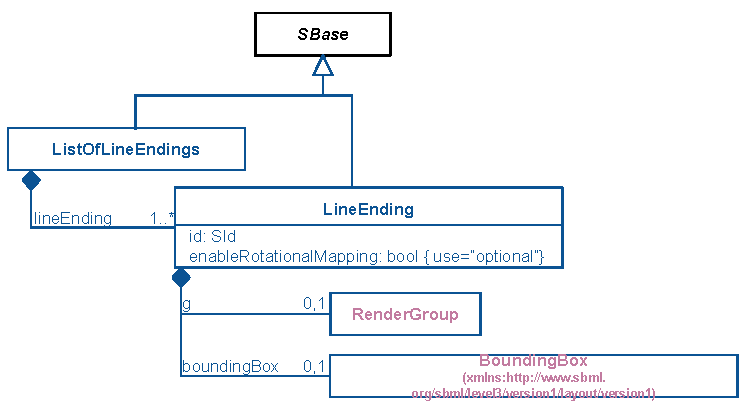
\includegraphics{images/render-line-endings-uml}\\
  \caption{A UML representation of the \LineEnding class for the \RenderPackage.  See \ref{conventions} for conventions related to this figure. }
  \label{fig:line_ending_render_uml}
\end{figure}


The \LineEnding object derives from the \GraphicalPrimitiveTwoD class
and thus inherits any attributes and elements that are present on this
class.
A \LineEnding contains exactly one \class{BoundingBox} element from the \LayoutPackage which allows the \token{position} and \token{dimensions} to be specified. It also contains a \RenderGroup element which provides the necessary render information for the line ending.
  
In addition the \LineEnding object has the a required \token{id} attribute and an optional \token{enableRotationalMapping} attribute.

\paragraph{The \fixttspace\token{id} attribute}

A \LineEnding has a required attribute \token{id} of type
\primtype{SId} which allows a unique identifer to be provided for this \LineEnding so that it may be referenced by other objects. The \token{startHead} and \token{endHead} attributes on a \RenderCurve expect to point to the \token{id} of a \LineEnding.

\begin{figure}[!h]
\begin{center}
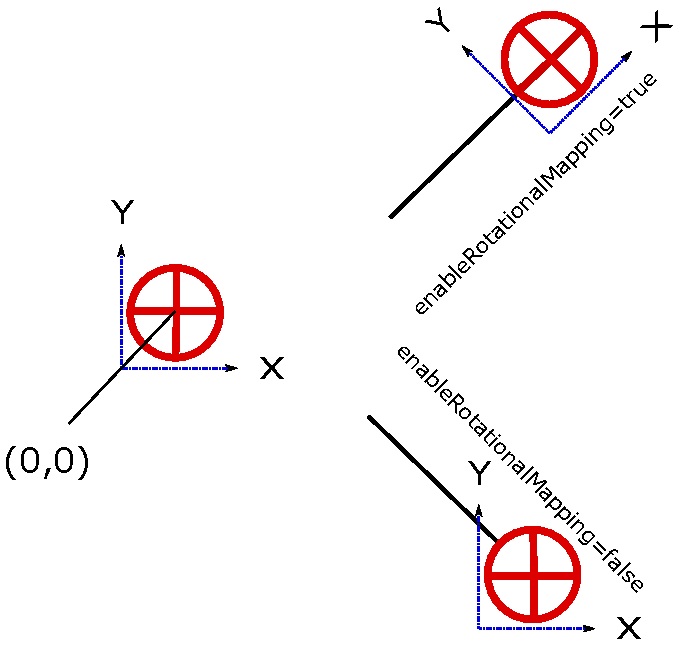
\includegraphics{figures/EnableRotationalMapping.pdf}
\end{center}
\caption{example of a line ending with and without rotation mapping enabled}
\label{EnableRotationalMapping}
\end{figure}

\paragraph{The \fixttspace\token{enableRotationalMapping} attribute}

A \LineEnding has an optional attribute \token{enableRotationalMapping}
of type \primtype{boolean} which specifies whether a line ending
will be rotated depending on the slope of the line it is applied to (if \val{true}) or if it is
drawn just the way it was specified (if \val{false}).


It should be noted that the top level \RenderGroup in a \LineEnding differs from top level groups in normal graphical elements in one respect; that is, the top level \RenderGroup of a \LineEnding inherits all attributes from the line it is applied to except for the attributes for the line endings themselves. This way a style sheet can define one line ending which can be applied to lines of different colors and it inherits the color from the line.
If the group also inherited the attributes for the line endings and it contained a \texttt{curve} element itself, we would have generated an endless loop.

The example snippet shows the definition of an arrow head.
\pagebreak
\exampleFile{examples/example_lineending.xml}


